\section{Introduction}\label{sec:intro}



%%\subsection{Problem Description}


Developers often use online question and answering (Q\&A) forums,
e.g., StackOverflow (S/O), to learn how to use software libraries and
frameworks. Sometimes, the answer to a question comes as a
fragment/chunk of code, which later makes it to the production
applications, stemming from the copy-and-paste software reuse
practice. Unfortunately, if the copied code fragments are vulnerable,
i.e., possess defects that can potentially be exploited, it will lead
to the applications being prone to attacks. Verdi {\em et
  al.}~\cite{verdi-tse22} reviewed more than 72K C++ code snippets
that migrated from 1,325 S/O answers. Of these, they reported a total
of 99 vulnerable code snippets of 31 different types that made their
way to 2,589 GitHub repositories. Thus, it is crucial to detect early
the vulnerabilities in the code snippets from online forums.
%Running a vulnerability detection tool on the source code after the
%integration of a S/O code snippet into the current codebase would
%waste developers' effort for such integration.

Security researchers have proposed several automated approaches for
vulnerability detection (VD) using program
analysis~\cite{FlawFinder,RATS,viega2000its4,Checkmarx,HPFortify,Coverity,BufferOverFlow,SQLInj,Cross-siteScripting,AuthBypassSpoofing},
as well as machine learning (ML) including deep learning
(DL)~\cite{fse21,chakraborty2020deep,zhou2019devign,li2018sysevr,li2018vuldeepecker}
techniques. However, these approaches warrant the code to exist as
complete program units, often making use of program representations
such~as abstract syntax tree (AST), Program Dependence Graph
(PDG)~\cite{fse21,li2018vuldeepecker}, Control Flow Graph
(CFG)~\cite{zhou2019devign}, Data Flow Graph
(DFG)~\cite{zhou2019devign}, Code Property Graph
(CPG)~\cite{chakraborty2020deep}, etc. At a minimum, they operate at
the method-level granularity, making it impossible to utilize them for
directly detecting vulnerabilities in code snippets. A possible
alternative would be to plug the code snippet into the method, resolve
any ambiguities, and test it with a VD tool. However, such a strategy
is limited. First, if found vulnerable, the efforts of integrating the
code snippet into the existing method would be lost. Second, due to
the black-box
%(inexplicable?)
nature of DL models, we would not know the origin of the
vulnerability, i.e., whether it arises due to the flawed code snippet
or the existing part of the code.

%other statements in the method.

%Besides, even a commit-level VD model requires the code before/after changes to be syntactically valid to extract those features.

Importantly, analyzing code snippets is not straightforward as they
are often incomplete, un-parseable, contain declaration/reference
ambiguity, and are interspersed between user comments. Currently,
there exist tools such as PPA~\cite{ppa08},~which parse an incomplete
code fragment to build the AST and~ex\-tract data types in a
best-effort manner, while StaType \cite{icse18} resolves the libraries
and recovers only the fully-qualified names for references. However,
the basic infrastructure for partial program analysis on incomplete
code snippets is not yet possible. The infrastructure includes the
fundamental supports/services such as lexical, syntactic, and semantic
analysis so that the static and dynamic analysis techniques could be
built upon. Let us call such an infrastructure, {\em partial program
analysis infrastructure}.

In addition to vulnerability detection, such partial program analysis
infrastructure is also beneficial to the other software engineering
(SE) tasks that can tolerate a low level of errors and imprecision in
building the program representations. For example, consider code
completion~\cite{codefill-icse22,facebook-icse21}, in which a model
provides suggestions to complete partial code. Existing ML/DL-based
code completion models are just based on the code sequences or utilize
the syntactic structure in ASTs, but none leverage the program
dependencies due to the nature of partial code. Next, consider the
task of analyzing the code fragments in a bug report to connect it to
the relevant source files for bug localization
purposes~\cite{euler-fse19,icpc17}. Here too, a need for partial
program analysis, especially for partial program dependence analysis,
can be observed.









%\section{Introduction}
\subsection{Problem Description}

%\url{https://www.nsf.gov/funding/pgm_summ.jsp?pims_id=503286}

%NSF: Smart city digital twins (Ray: to speak to San Antonio city CIO) + below


%{\em Develop integrated, automated methods for detecting and responding to cyber-security vulnerabilities and compromise. The solution would ultimately have thresholds for AI/ML responses versus those that require a human in the loop. It would also select the most appropriate action and quantify the impact of that action to achieve intended end states. While solutions that only address particular aspects (such as automated detection, response, and remediation) are acceptable, the ultimate goal is an integrated suite of solutions.}

The need for cyber resilience is increasingly important in our
technology-dependent society, where computing systems, devices and
data have been, and will continue to be, the target of cyber
attackers, particularly advanced persistent threat (APT) and
nation-state / sponsored actors. For example, an individual pleaded
guilty to participating in a distributed denial of service attack
carried out by infecting compromised IoT devices with the Mirai
malware, which impacted a domain name resolver that subsequently
affected the websites of Sony, Twitter, Amazon, PayPal, Tumblr,
Netflix, and Southern New Hampshire University with lost advertising
revenues and remediation costs. Among them, Sony estimated that "its
resultant losses included approximately \$2.7 million in net
revenue"~\cite{USDoJMirai2020}. However, APT and
nation-state/sponsored actors tend to be more sophisticated and have
access to significantly more resources and time to facilitate their
attacks, which in most cases are not financially driven (unlike
typical cyber criminals). For example, the cyber security research
community have reported observations of “false flag” cyber
operations \cite{geers2014world,Leyden2019}, where an attack is staged
by sophisticated attackers (e.g., APT actors) in such a way to mislead
the intended victims into believing that another party (e.g., another
nation/state) is responsible for the cyber attacks, e.g.,~by using or
mimicking ``the tools, techniques, and even languages typically used
by the group or country the attackers are trying to
frame'' \cite{Fruhlinger2020}.
%We also posit the importance of digital forensics (often considered to
%be reactive) in human-in-the-loop cyber threat intelligence and
%hunting solutions, as digital (forensic) investigations can also
%facilitate attribution (tracing and identifying the attack source),
%and help to answer the six key questions – {\em what, why, how, who,
%when, and where} – of an incident occurrence.
As an example, the SolarWinds attack was first discovered by the
cybersecurity firm FireEye in December 2020, who reportedly found
unusual data being sent to a server of unknown
origin \cite{FireEyeUNC2452}. Upon further digital forensic
investigations, it was uncovered that one of the servers that provides
access to updates and patches for SolarWinds Orion tools was
compromised, thus allowing the attackers to inject code into the
software updates and infect multiple clients. The malicious code
allowed data modification and exfiltration and remote access to
devices that had the software installed. Based on the forensic
investigations, the Cyber-security and Infrastructure Security Agency
released a summary of tactics, techniques, and procedures associated
with the incident~\cite{CISA2021}.

While there are a broad range of commercial security information and
event management (SIEM) systems, and other security orchestration,
automation, and response (SOAR) solutions
(see \cite{DBLP:journals/csur/IslamBN19} for an overview of SOAR
solutions), a 2021 Gartner report observed that ``Security and risk
management leaders are struggling with too many security tools from
different vendors with little integration of data or incident
response'' \cite{FirstbrookLawsonGartner2021}. The same report also
noted the increasing importance of having in place ``a unified
security incident detection and response platform that automatically
collects and correlates data from multiple proprietary security
components''.

There are, however, a number of challenges we need to address in the
design of a system to facilitate automated vulnerability detection.
For example, an automated security vulnerability detection tool often
runs as follows. First, a user runs the tool on the software to be
analyzed. Then, the tool will report the potential vulnerabilities
that it detects in the software. Finally, the user or a software
analyst will go through the report and examine the potential
vulnerabilities. A tool is considered as accurate if the vulnerability
it reports is actually vulnerable. It is considered as having high
coverage if it can cover and reveal all the vulnerabilities in the
software / hardware. Balancing coverage and accuracy involves an
inherent trade-off. The tool can list only true-positives (low
coverage, high accuracy), or it can output all potential anomalies
(high coverage, low accuracy). Achieving both high coverage and high
accuracy in a fully automated tool can be impossible or prohibitively
expensive, in terms of implementing the automation and/or sifting
through the large number of erroneous results manually.
%This is true for an IoT system with complex software and hardware
%integration.
Also, what is considered malicious in one application may be
considered benign in another due to differences in the purpose and the
context of these applications. For example, accessing of contacts by
an e-mail client is a legitimate operation, but it is illegitimate,
and probably malicious, in a surveillance camera
application. Importantly, malicious activities and operations
frequently blend their overt and malicious purposes. For example, an
surveillance camera recording the regular activities at an ATM machine
can leak the recordings to a malicious server without the knowledge of
the users, which can be abused to steal the
identification/passcode. Hence, there is a need to integrate
artificial intelligence (AI; broadly defined to include both machine
and deep learning) techniques to facilitate the identification of
adversarial, anti-security and anti-forensics activities and
techniques. A 2020 report by Gartner, for example, suggested that
``[b]y 2022, 40\% of machine learning~model development and scoring
will be done in products that do not have machine learning as their
primary goal'' \cite{RichardsonGartner2020}.

%Automating identification of malicious activities in large-scale IoT systems may require a large number of specific features and incur significant computation cost. In contrast, using automated tools for simple cases and leaving all the complex ones for a user to resolve is also not practical. We also note that AI techniques can facilitate the development, understanding, interpretation, and sharing of analytic content (collectively referred to as augmented analytic). Hence, this reinforces the importance of Human-in-the-Loop cyber threat intelligence and hunting solutions, which integrates information obtained from different systems. This provides the motivation and inspiration of this proposal. 

Another key challenge with the state-of-the-art AI/ML-based
vulnerability detection approaches is the lack of explanation on why
the model determines the vulnerable code. They resolve complex
scenario of security vulnerabilities as an output of an AI/ML model
(e.g., a definitive outcome of yes or no, or a likelihood score for
vulnerability degree). This hinders the understandability of the
output. Developers would not know why the model makes that decision,
and do not know where and what to look for and to fix the
vulnerability in their code.

In this proposal, we focus on two key factors, namely: automated AI/ML tools and human analysts. There exists some defined threshold for AI/ML solutions versus those that require human intervention. In \emph{ordinary scenarios}, the cost and complexity of the solutions are both low. Either human analysts or automated tools can handle them with minimal effort. However, the {\em automation wall} exists for \emph{complex scenarios} in which the cost for resolving complex scenarios escalates beyond that wall.




\subsection{Goals and Objectives}
%The objective is ``\textbf{Automated Risk Detection and Mitigation}''

In this proposal, we propose XAI-enabled Vulnerability Detection and
Assessment Framework (XAI-VDA). Instead of resolving complex scenarios
of security vulnerability detection as an binary output of yes and no,
we aim to leverage Explainable AI to amplify the human intelligence in
detecting vulnerabilities and assessing their impacts in software
systems.

In our proposed `Human-in-the-Loop Explainable-AI-Enabled
Vulnerability Detection, Investigation, and Mitigation' (HXAI-VDIM)
system, instead of resolving complex scenario of security
vulnerabilities as an output of an AI/ML model (e.g., a definitive
outcome of yes or no, or a likelihood score for vulnerability degree),
we integrate the security analyst or forensic investigator into the
man-machine loop and leverage the explainable AI (XAI) to combine AI
and Intelligence Assistant (IA) in amplifying human intelligence in
both proactive and reactive processes. Our philosophy is that {\em "a
  machine and a mind can beat a mind-imitating machine working by
  itself"}~\cite{DBLP:conf/ifip/Brooks77}. Our ultimate goal is that
the proposed HXAI-VDIM system will amplify the human intelligence in
resolving and investigating complex security vulnerabilities. In other
words, HXAI-VDIM integrates both human and machine in an interactive
and iterative loop that utilizes human intelligence to guide the
XAI-enabled system and generate refined outputs -- see Figures
\ref{fig:overview} and \ref{fig:arch}.

Specifically, HXAI-VDIM's workflow is as follows. The Explainable Detection Model is trained via the dataset collected throughout the operations of the system (and in the context of our proposal, IoT system) as well as those from other sources. The trained model is then used to run on the current IoT system. The result of the XAI model will be visualized through a Security Vulnerability Visualization (SVV) model to produce for the human expert the report of observable evidences on the potential vulnerabilities in the IoT system under study.  
Unlike traditional ML model, the Explainable Detection model used for vulnerability detection, investigation, and mitigation (VDIM) {\em produces not only the detection results but also the connections between the results and the input IoT system indicating the reasons why the model has made that decision}. Specifically, the observable evidences will point to the specific data collected from the potentially vulnerable components (hardware and/or software) in the IoT system that are crucial for the XAI model to come up with the result. For example, in the smart campus IoT system, at the first iteration, the XAI model can point to a long list of different potentially vulnerable components as the root causes. Unlike in the traditional approach where the human expert will sift through the long list with several false negatives, (s)he will be integrated into the VDIM process for the next iteration. The human expert will compare the observable evidences with the potential vulnerabilities identified in the previous iteration to provide the adjustments on those identified vulnerable components. Based on those adjustments, the input to the XAI model in the next iteration will be modified accordingly as well as the parameters of the XAI-enabled Detection Model. The entire process of HXAI-VDIM is repeated until all (detected) vulnerabilities are identified or the human expert is confident about the given system. For security investigation, the forensic expert or security analyst will consult with the observable evidences to produce the final report on the vulnerabilities.


%\begin{wrapfigure}{l}{0.8\textwidth}
\begin{figure}[t]
	\centering
	\includegraphics[width=4in]{hxai-vdim.jpg}
	\caption{Human-in-the-Loop XAI-enabled Vulnerability Detection, Investigation, and Mitigation}
	\label{fig:overview}
\end{figure}
%\end{wrapfigure}
With the Human-in-the-Loop framework, the two key stakeholders (human expert -- forensic investigator and/or security analyst, and automated tool) {\em complement  each other} in producing an effective and efficient VDIM process. {\em The automated tool leverages human intelligence to quickly narrow down the features/factors crucial for the tool. At the same time, human intelligence is amplified with the use of automated tool via XAI and visualization}. To realize our framework, we will pursue the following three key work tasks.

\noindent {\bf Work Task 1. HXAI-VDIM System Design and Implementation} (Section~\ref{section:T1}). In this work task, we will design and develop our HXAI-VDIM architecture to be concretized into a tool-suite of supports on (1) security vulnerability detection that pro-actively scans the potential risks and vulnerabilities; (2) security vulnerability investigation toolset that assists forensic analysts and experts in performing digital (forensic) investigations, tracing, and identifying the attack source of an incident occurrence; and (3) an integrated tool suite for the remedial and mitigation actions in the wake of such security incident.


\noindent {\bf Work Task 2: Proactive Human-in-the-Loop Vulnerability Detection with Explainable AI} (Section~\ref{section:T2}). In this work task, we will design and develop the core components relevant to proactive direction of our HXAI-VDIM architecture. First, we will develop the theoretical framework,
algorithms, and models for proactive vulnerability detection to identify the vulnerable IoT devices in an IoT network. Second, we will investigate and design the XAI model that will provide the vulnerability detection results on the vulnerable IoT devices, and explain why the model predicts such a vulnerability by making connections from the result to the input for such an explanation. Finally, we will develop a Human-in-the-Loop framework that leverages the XAI-based vulnerability detection model to realize our HXAI-VDIM framework shown in Figure~\ref{fig:overview}.  

\noindent {\bf Work Task 3: Human-in-the-Loop, XAI-enabled Digital Forensic Investigation and Mitigation} (Section~\ref{section:T3}) In this work task, we will design and develop the core components relevant to forensic investigation and mitigation (reactive activities). The first module is the software vulnerability scanner. After the vulnerable IoT device is identified and isolated, we start scanning for software vulnerabilities in each isolated device. After software scanning, the forensic expert will use our XAI model to perform forensic investigation and start the mitigation process as needed. Thus, the second module in this work task is the Human-in-the-Loop framework for forensic investigation that is guided by the XAI-enabled Vulnerability Detection Model.

\subsection{NSF Research Objectives and Anticipated Results}

\begin{figure}[t]
    \centering
%    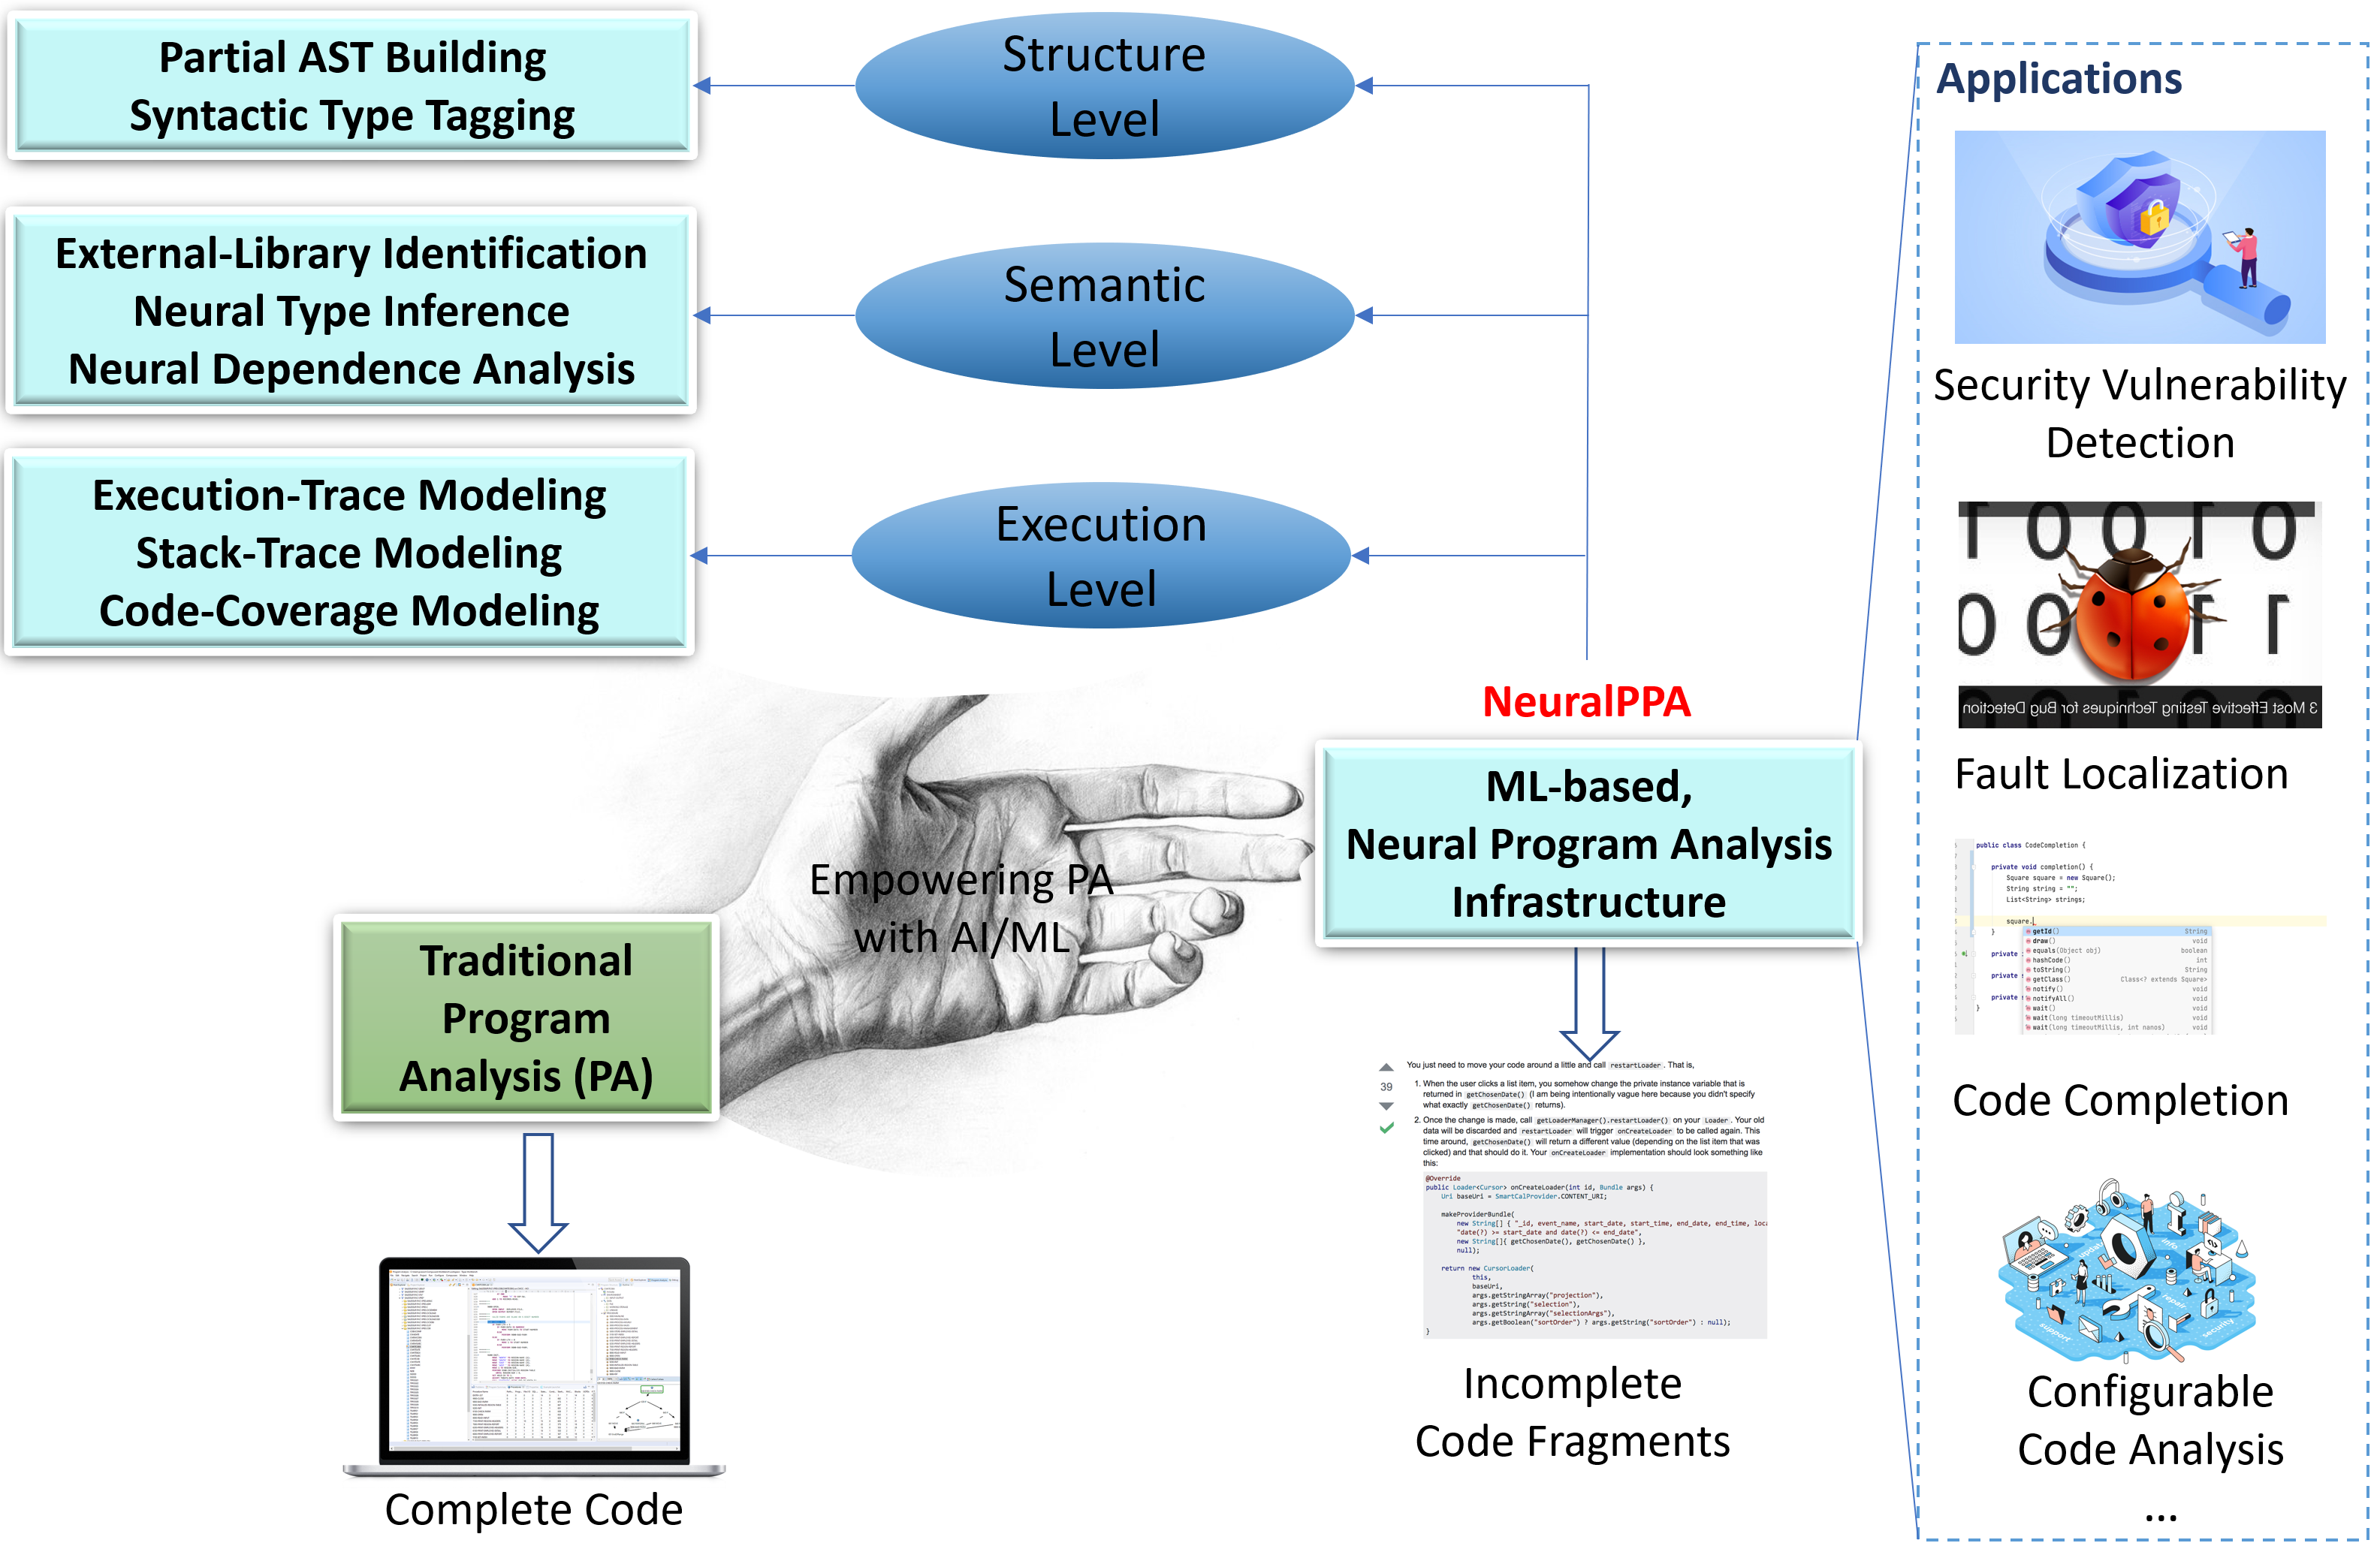
\includegraphics[width=0.83\textwidth]{graphs/neuralppa}
    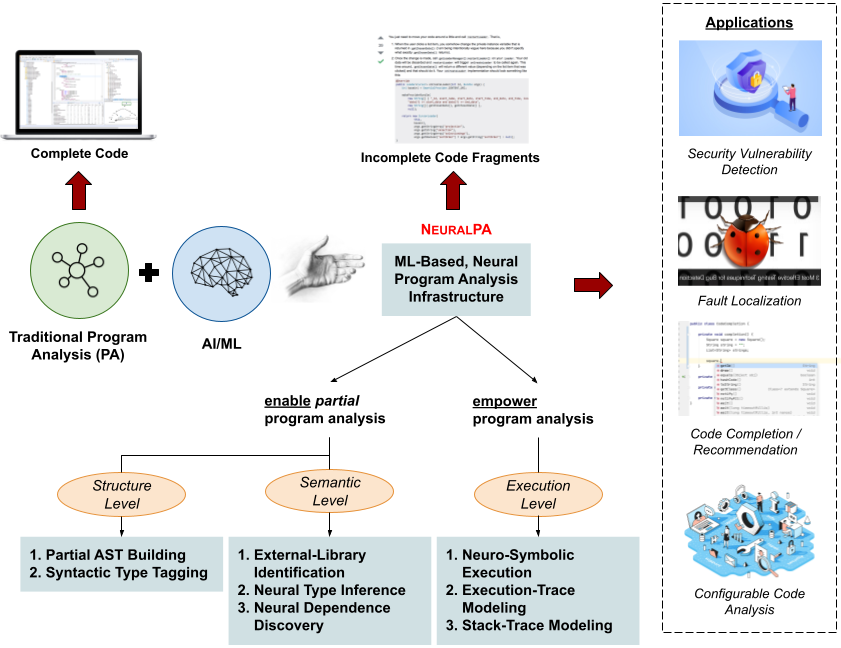
\includegraphics[width=0.92\textwidth]{figures/infra-design-3.png}
%    \vspace{-10pt}
    \caption{{\tool}: Machine Learning-based Program Analysis Infrastructure}
    \label{fig:arch}
\end{figure}


In this proposal, we seek to address these issues and advance the state-of-the-art in traditional program analysis by means of {\tool}, a {\em \underline{Neural} Network-Based \underline{P}rogram \underline{A}nalysis} infrastructure. We aim to establish {\em a scientific foundation, novel methodologies, frameworks, models, and algorithmic solutions for neural program analysis}. Our primary focus areas can be summarized as follows: 

%(1) {\bf Enabling analysis of incomplete code fragments}, i.e., partial program analysis;
(1) {\bf enabling analysis of incomplete code fragments}, i.e., partial program analysis;

%(2) {\bf Empowering existing PA tools by making them more sound and complete}. 
(2) {\bf empowering existing PA tools with advanced AI/ML
%techniques
} to make them more sound and complete.

\noindent Figure~\ref{fig:arch} illustrates the 
%general 
framework for {\tool}, which will allow the construction of efficient program analysis techniques for (partial) code, also based on which downstream 
%software engineering 
SE applications can be built.


\begin{center}
    \begin{minipage}{36em}
The key philosophy that drives our work is that the {\em structural, semantic, and symbolic execution-level analyses of partial code can be learned from the analysis of entire programs in the wealth of information obtained from ultra-large-scale, open-source software repositories}.
    \end{minipage}
\end{center}



We draw motivation for such a data-driven, learning-based approach from the following. First, ultra-large-scale software repositories, e.g., GitHub (7M+ projects) and SourceForge (700k+ projects), contain an enormous collection of programs. These repositories amount to 1B+ lines of code, 10M+ revision logs, and 3M+ issue reports. This wealth of knowledge is an excellent source for {\tool}. Hindle {\em et al.}~\cite{naturalness-icse12} have shown that code has high repetitiveness and predictability and can be captured well by statistical models. Thus, we expect to build ML/DL models to learn from those repositories. 
Second, the PI group reported a high repetitiveness level for AST code structure in open-source projects~\cite{icse15}. Thus, {\tool} infrastructure could help learn structure-level information from the ASTs extracted for whole programs in the existing code repositories and infer data types, partial ASTs for partial programs. Third, in an empirical study on the repetitiveness, containment, and composability of PDGs in open-source projects, the PI group~\cite{msr16} reported that among 17.5M PDGs with 1.6B PDG subgraphs, 14.3\% of the PDGs have all of their subgraphs repeated across different projects. Furthermore, in 15.6\% of the PDGs, at least 90\% of their subgraphs are likely to have appeared before in other projects. 
%Thus, {\tool} could learn from PDGs with complete program dependencies retrieved from existing code repositories and derive the dependencies for the (partial) code fragment under study. The PI group also reported a high repetitiveness level for AST code structure in open-source projects~\cite{icse15}.
Thus, {\tool} could learn semantic-level information from the PDGs with complete program dependencies retrieved from existing code repositories and infer such dependencies for the partial code fragment. Execution can also be modeled
from the ones in the past.

%\textcolor{red}{Add a line for execution-level}.

%Finally, such a program analysis infrastructure like {\tool} can be
%drawn from the spirit and successes of the approaches in natural
%language processing (NLP). For example, at the lexical level, the task
%of deriving the token types for source code tokens could be analogous
%to the part-of-speech (PoS) tagging in NLP. At the syntax level, the
%task of learning the syntactic structure in AST of the partial code
%can be inspired by the approaches to build parse trees for
%natural-language texts. At the semantic level, the partial program
%dependence analysis infrastructure is similar in spirit to the neural
%network-based dependency parsing in NLP, which learns the dependencies
%signifying the semantic relationships between words in a sentence from
%text corpora. In addition, there is much room for innovations in AI/ML
%for source code.

Broadly, the proposed program analysis infrastructure, \tool, draws inspiration from the successes of the neural network-based approaches in the field of natural language processing (NLP). For example, the task of deriving the data types for the source code tokens is analogous to the part-of-speech (POS) tagging task in NLP. At the syntactic level, learning the syntactic structure, i.e., the ASTs for partial code can be inspired by the approaches to infer parse trees for natural language texts. At the semantic level, the partial program dependence analysis infrastructure is similar in spirit to neural network-based dependency parsing in NLP, which learns the dependencies signifying the semantic relationships between words in a sentence from text corpora. In addition, there is much room for innovations in AI/ML for source code.


To accomplish these tasks, we propose the following thrusts of research in {\tool} (see Table~\ref{tab:milestones}):

\vspace{3pt}
%\noindent \textbf{Thrust 1. Neural Structural Analysis Infrastructure
%  \code{NeuralStruct}.} ({\em Section~\ref{}}) Source code has
%well-defined structures and semantics. Thus, the basic infrastructure
%in {\tool} is the neural structural analysis component.  This
%component has two main tasks. First, it learns from the syntactic
%structures of the complete code in the training dataset collected from
%large-scale code repositories, to derive the abstract syntax tree
%(AST) that best represents the syntactic structure of the given
%partial code, i.e., with the highest likelihood/probability.  The
%traditional lexical analyzer still works for partial code due to the
%independence nature of lexical tokens. The second task of this
%component is to tag the code tokens with the types of the syntactic
%units including the statement types (\code{if}, \code{for}, etc.),
%variables, fields, methods, classes, etc. Both of the tasks can be
%performed with our learning-based approaches in a dual-learning
%manner.

\noindent \textbf{Thrust 1. Neural Structural Analysis Infrastructure.} ({\em Section~\ref{sec:thrust1}}) Source code has a well-defined structure and semantics. Thus, the basic infrastructure in {\tool} is the neural structural analysis component, which primarily has two tasks. First, it learns from the syntactic structures of the complete code in the training dataset collected from large-scale code repositories, to derive the abstract syntax tree (AST) that best represents the syntactic structure of the given partial code, i.e., with the highest likelihood/probability. The traditional lexical analyzer still works for partial code due to the independence nature of lexical tokens. The second task of this component is to tag the code tokens with the types of the syntactic units including the statement types (\code{if}, \code{for}, etc.), variables, fields, methods, classes, etc. Both of the tasks can be performed with our learning-based approaches in a dual-learning manner.
  
\vspace{3pt}
\noindent \textbf{Thrust 2. Neural Semantic Analysis Infrastructure.}
({\em Section~\ref{sec:thrust2}}) The basis components for several
analysis techniques on the semantics of the program include the
following:

1) the identification of the APIs of the external libraries in the
external references in the partial code: this is needed because the
partial code contains the undeclared reference and/or
declaration/reference ambiguity without explicit declaration of the
APIs in the external libraries.

2) the inference of the type information for the entities in the
partial code: due to the ambiguity in the declaration, the types of
the variables and statements are not always obviously
identified. Thus, the type inference is a basic service within
{\tool}.

3) the inference of the program dependencies among the statements in
the partial code: several program analysis techniques are based on the
program dependencies, which are not always obtainable due to the
incompleteness of the given code fragment.

\vspace{3pt}
\noindent \textbf{Thrust 3. Neural Symbolic Execution Infrastructure.}
({\em Section~\ref{sec:thrust3}})
Symbolic execution is a means of analyzing a program to determine what
inputs cause each part of a program to execute. Symbolic execution
performs executing a program abstractly, so that one abstract
execution covers multiple possible inputs, which are assumed to have
symbolic values. We aim to explore the novel area in AI named
neuro-symbolic learning, which seeks to combine traditional
rules-based AI approaches with modern deep learning techniques.  We
will leverage traditional program analysis rules to enhance the
learning of the characteristics on the execution of the partial code
fragment.

\vspace{3pt}
\noindent \textbf{Thrust 4. Neural Partial Program Analysis
  Applications.}  ({\em Section~\ref{sec:thrust4}}) Our last thrust of research
is aimed to evaluate our basic partial program analysis infrastructure
in a few applications. The following software engineering
applications could be our examples: 1) software vulnerability detection for code snippets,
2) fault localization, and 3) code completion.

%\vspace{3pt}
%\noindent \textbf{Thrust ???. Neural Execution Analysis Infrastructure.}
%({\em Section~\ref{}}) All the dynamic analysis techniques require the
%analysis and understanding of the execution. However, for an
%incomplete code, we first need to design a component that can wrap
%around the given code fragment with the minimum code so that the code
%fragment can be executed. When the code is executed, we also need the
%approaches that represent the executed statements and their relations,
%model the execution and stack traces, and model the code coverages
%for an execution.


\begin{table*}[t]
	\vspace{-15pt}
\begin{center}
{\footnotesize{
\begin{tabular}{cc}
\begin{tabular}[t]{|p{0.2in}|p{2.95in}|} 
\hline
\multicolumn{2}{|>{\columncolor[gray]{0}}c|}{\textcolor{white}
{\bf Year 1 Project Milestones \& Deliverables}}\\
\hline 
\hline
\multicolumn{2}{|c|}{\bf T1. Neural Structure Analysis Infrastructure}\\
\hline
{\bf 1.1} & Neural Syntactic Type Tagging\\
{\bf 1.2} & Neural Partial AST Building\\
{\bf 1.3} & Evaluation of the components\\
\hline
\hline
\multicolumn{2}{|c|}{\bf T2. Neural Semantic Analysis Infrastructure}\\ 
\hline
{\bf 2.1} & External-Library Identification\\
\hline
%\hline
%\multicolumn{2}{|c|}{\bf Integrate Code Synthesis into Tools}\\
%\hline
%{\bf 1.5} & \goalOneFour.\\
%\hline
\multicolumn{2}{c}{}
\end{tabular}
&
\begin{tabular}[t]{|p{0.2in}|p{2.95in}|} \hline
\multicolumn{2}{|>{\columncolor[gray]{0}}c|}{\textcolor{white}
{\bf Year 2 Project Milestones \& Deliverables}}\\
\hline 
\hline
\multicolumn{2}{|c|}{\bf T2. Neural Semantic Analysis Infrastructure}\\
\hline
{\bf 2.2} & Neural Type Inference\\
{\bf 2.3} & Neural Dependence Analysis\\
%{\bf 2.3} & Integrate Evaluation Framework into Design Environment\\
%{\bf 2.4} & Evaluate CRL Framework with Existing Models\\
%{\bf 2.3} & \goalTwoThree.\\

\hline
\hline
\multicolumn{2}{|c|}{\bf T3. Neural Execution Analysis}\\ 
\hline
%{\bf 3.1} & Design New Code Representations and Learning Models.\\
{\bf 3.1} & Neural Execution-Trace Modeling\\
%{\bf 2.4} & Advance FL and RT-CI Approaches.\\
%{\bf 2.5} & Advance Regression Testing in CI Approaches.\\
%{\bf 2.5} & Advance APR Approaches with Framework.\\
\hline
%\hline
%\multicolumn{2}{|c|}{\bf Community Involvement: Capacity Building}\\
%\hline
%{\bf 2.4} & \goalTwoFour.\\
%{\bf 2.5} & \goalTwoFive.\\
%{\bf 2.6} & \goalTwoSix.\\
%\hline
\multicolumn{2}{c}{}
\end{tabular}
\end{tabular}\\
\vspace*{-.3cm}
\begin{tabular}{c}\hline
\multicolumn{1}{|>{\centering\columncolor[gray]{0}}p{6.44in}|}{\textcolor{white}
{\bf Year 3 Project Milestones \& Deliverables}}\\
\hline
\end{tabular}\\
\vspace*{-.2cm}
\begin{tabular}{cc}
\begin{tabular}[t]{|p{0.2in}|p{2.95in}|}
\hline
\multicolumn{2}{|c|}{\bf T3. Neural Execution Analysis}\\
\hline
{\bf 3.2} & Neural Stack Trace Modeling\\
{\bf 3.3} & Neural Code Coverage Modeling\\

%{\bf 3.3} & Testing on Models in IDE tools.\\
\hline
%\hline
%\multicolumn{2}{|c|}{\bf \goalTwo}\\ 
%\hline
%{\bf 3.3} & \goalThreeThree.\\
%\hline
\multicolumn{2}{c}{}
\end{tabular}
&
\begin{tabular}[t]{|p{0.2in}|p{2.95in}|}
\hline
\multicolumn{2}{|c|}{\bf T4. Neural Partial Program Analysis Applications}\\
\hline
%{\bf 3.1} & Design New Code Representations\\

{\bf 4.1} & Security Vulnerablity Detection with {\tool}\\
{\bf 4.2} & Fault Localization and Completion with {\tool}\\

\hline
\multicolumn{2}{c}{}
\end{tabular}
\end{tabular}
\vspace{-15pt}
}}
\end{center}
\vspace*{-.3in}
%\caption{Tasks and Milestones. (Rep. = Representation)}
\caption{The 3-year schedule of Thrusts, Tasks, and Milestones of this proposal.}
%the schedule of Thrusts, Tasks, and Milestones of this proposal.
%\vspace{-10pt}
\label{tab:milestones}
\vspace{-10pt}
\end{table*}
%


Toward this theme, in our preliminary work, we developed DeepPDA
(Section~\ref{sec:deeppda}), a neural network-based partial program
dependence analysis approach that learns to derive the program
dependencies for any code fragments (i.e., both complete and
incomplete). In our preliminary empirical evaluation, we intrinsically
evaluated it on Java and C/C++ programs. We trained DeepPDA on
complete code. For testing, we treated each method individually and
chose a consecutive portion within the method to predict the program
dependencies, and compared them against the actual
dependencies. Overall, DeepPDA predicts CFGs/PDGs in Java with
an F-score of 94.29\%, and in C++ with an F-score of 92.46\%. As
another preliminary work (Section~\ref{sec:statype}), we also
developed an approach to derive the data types of the variables in the
code snippets. We treat the problem as statistical machine translation
from source code with partially qualified names to source code with
full names. Our preliminary evaluation on StackOverflow posts shows
that our technique achieves high accuracy with 97.6\% precision and
96.7\% recall in deriving data types in code snippets.



%\subsection{Significance of This Proposed Project: NSF Merit Criteria}

\section{Intellectual Merits}

The results of this project will advance the state-of-the-art
knowledge and scientific foundations in both software security and
machine learning (explainable AI). They are transformative and
directly help improve software quality with novel automated software
vulnerability detection and assessment techniques.

\noindent \underline{{\bf Advance the state-of-the-art knowledge and
    understanding}}. Explainable AI-enabled vulnerability detection in
both binary and source code in Thrusts 1 and 3 will advance the body
of knowledge and theoretical foundations for both areas of machine
learning for code and software security. Thrust 2 will also help
advance the practical tools in software security and engineering.

\noindent \underline{{\bf Scientific foundation, creative/original
    research}}. This project will provide a scientific foundation
(novel concepts, representations, algorithms, models, and tools) (1)
to enable the explanations for ML models in vulnerability detection,
(2) to empower the ML-based vulnerability detection and assessment.

%and (3) to enable the applications of program analysis on incomplete
%code such as vulnerability detection on code snippets, code
%completion, etc.

\section{Broader Impacts}

\underline{{\bf (1) Transformative and benefits to society}}. Our
results will be transformative and directly benefit to our society.
They will lead to increasing software quality \& reliability, software
security.  Our validation involves students and professionals,
promoting teaching, training, and learning of both {\bf software
  security} and {\bf machine learning} techniques that have wide
impacts in industry and academic communities.

\noindent\underline{{\bf (2) Foster other related research
    activities}}. Our results will foster {\em research activities in
  related fields of {\bf explainable AI/ML} and {\bf software
    engineering}}. We will produce theoretical concepts and techniques
that are novel in deep learning, e.g., XAI model for source and binary
code. The applications of our techniques in software engineering
applications will advance software security and reliability.

%The collected {\bf large scale bug\&fix corpus} will be useful for
%software quality and reliability research.
%Innovations in CRL could be used to {\bf advance other SE tasks}. We
%will also develop {\bf novel DL-based bug detect-fix} approaches.


\noindent\underline{{\bf (3) Education, dissemination, and broader participation}} (Section~\ref{edu}). The
research will enhance the infrastructure for teaching/research via
tools and data sets for use by students and practitioners, and for
enhancement by researchers. We will provide related learning
modules for educators as well. It will include outreach activities for
undergraduate students, underrepresented groups, minorities, and women
in science.
%contribute novel
%teaching modules to our curriculum.
%Details will be presented in Section~\ref{edu}



